%--------------------
% Packages
% -------------------
\documentclass[11pt,a4paper]{article}
\usepackage[utf8x]{inputenc}
\usepackage[T1]{fontenc}
%\usepackage{gentium}
\usepackage{mathptmx} % Use Times Font


\usepackage[pdftex]{graphicx} % Required for including pictures
%\usepackage[swedish]{babel} % Swedish translations
\usepackage[pdftex,linkcolor=black,pdfborder={0 0 0}]{hyperref} % Format links for pdf
\usepackage{calc} % To reset the counter in the document after title page
\usepackage{enumitem} % Includes lists

\frenchspacing % No double spacing between sentences
\linespread{2.0} % Set linespace
\usepackage[a4paper, lmargin=0.1666\paperwidth, rmargin=0.1666\paperwidth, tmargin=0.1111\paperheight, bmargin=0.1111\paperheight]{geometry} %margins
%\usepackage{parskip}
\usepackage{amsmath}

\usepackage[all]{nowidow} % Tries to remove widows
\usepackage[protrusion=true,expansion=true]{microtype} % Improves typography, load after fontpackage is selected
\usepackage{tabto}
\usepackage{apacite}
\bibliographystyle{apacite}
\usepackage{graphicx}
%\usepackage{lipsum} % Used for inserting dummy 'Lorem ipsum' text into the template
\graphicspath{ {./viz/} }
\usepackage[inkscapelatex=false]{svg}

%-----------------------
% Set pdf information and add title, fill in the fields
%-----------------------
\hypersetup{ 	
pdfsubject = {},
pdftitle = {},
pdfauthor = {Anita Sun}
}

%-----------------------
% Begin document
%-----------------------
\begin{document} %All text i dokumentet hamnar mellan dessa taggar, allt ovanför är formatering av dokumentet
\raggedright
\setlength{\parindent}{20pt}
\section{Mockup Data}

In my mockup results section, I first present a data structure visualization to aid in showing the shape of my dataset. The data structure visualization includes a truncated example of what data I will be using and how I will connect the relational data. We begin with the presidential candidate's verified campaign TikTok account and collecting all the follower accounts. From there, I will query followers' reposted TikTok videos as well as the other accounts that the user follows. From each reposted TikTok, I will gather video description information and hashtag information. Using this data, I will be able to conduct topic analysis and network analysis.

\includesvg[scale=0.8]{Data_Structure.svg}

\newpage

I also present several visualizations of a proxy dataset. This proxy dataset is a corpus of Donald Trump's Tweets from the end of 2016 until the start of 2021, retrieved from \href{https://www.thetrumparchive.com}{thetrumparchive.com}. This proxy dataset is an imperfect proxy; for example, it lacks the tree structure that my eventual dataset will have, and it is a case study of one social media account rather than many. However, I have been able to use some analysis techniques on the proxy dataset that I hope to eventually incorporate for my eventual real dataset.

This first visualization is a visualization of Trump's tweeting emotions over time as categorized by a pre-trained RoBERTa model. We can see that Trump's Tweeting frequency increased throughout the duration of his first presidential term. Tweets with ambiguous emotion or with sadness remain at comparatively low levels throughout this time period; however, we can see increases in volume of Tweets with anger towards the latter of this time period.

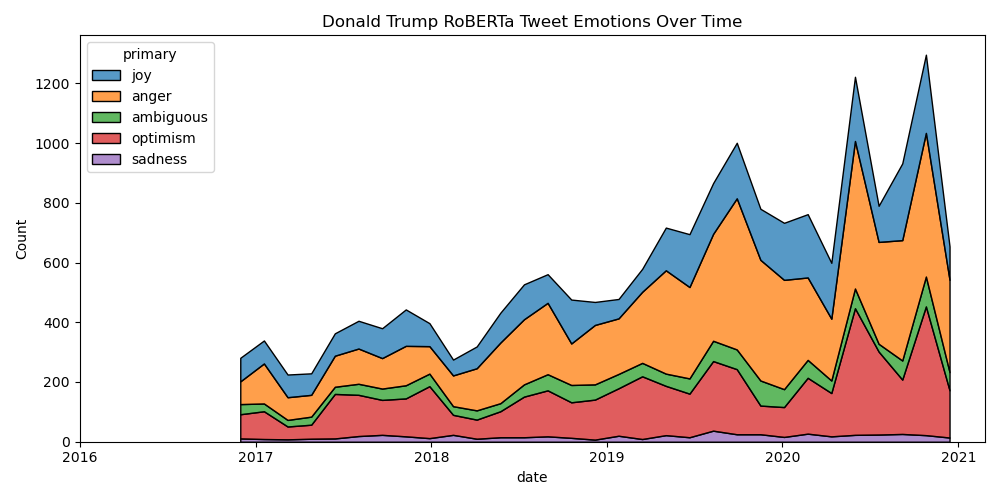
\includegraphics[scale=0.6]{viz/roberta_over_time.png}

\newpage
This next visualization is a similar visualization breaking down Trump's tweeting behavior by topic clusters. This topic clustering was performed using BERTopic, which is what I plan to use for eventual dataset. I have only included the eight most populated topics in my visualization to have more clarity and less clutter. You can see towards the end of 2020, Trump begins to tweet much more frequently about elections and ballots, which was well covered in mainstream media as he sowed distrust in the electoral process.

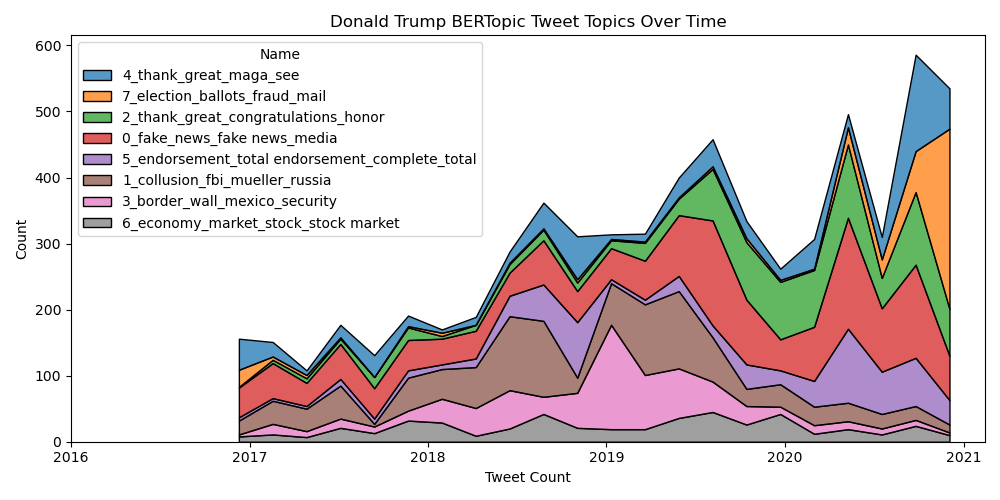
\includegraphics[scale=0.6]{viz/bertopic_over_time.png}

I have also experimented with ways to display social network data. Though this particular dataset does not lend itself to such diagrams, I am to generate a Sankey diagram that gives a precursor as to how I might approach displaying relational data. In the figure below, I show the cross distribution of emotions and BERTopic clusters. Though I have included this graphic here as an svg file, the plotly object is interactive in Python and has better visibility and dynacism. I simply add this visualization in this format as a proof of concept, and I would not utilize this format for a dynamic, interactive visualization.

\begin{figure}[t]
    \includesvg[width=\linewidth]{viz/emotion_topic_sankey.svg}
    \centering
    \caption{Caption}
    \label{fig:enter-label}
\end{figure}
%\includesvg[width=\pagewidth]{viz/emotion_topic_sankey.svg}

\end{document}